\providecommand{\main}{../..}
\documentclass[\main/thesis.tex]{subfiles}
\begin{document}

\section{Converting from Natural Numbers [work in process]}\label{fromnat}

\lstinline|Numeral| is a family of types, so as functions that are defined on
\lstinline|Numeral|.
It is important to regard functions such as \lstinline|⟦_⟧| as a collective;
each has a different configuration of indices.

Here, we name the fuction that converts natural numbers to corresponding
numerals \lstinline|fromℕ|.

\begin{center}
    \begin{tikzpicture}
        \matrix (m) [matrix of nodes,row sep=6em,column sep=8em,minimum width=4em]
            {
                {\lstinline|Numeral b d o|} & {\lstinline|ℕ|} \\
            };
        \path[-stealth]
            ($(m-1-1.east)+(0,+0.1)$)
                edge node [above] {\lstinline|⟦_⟧|}
                ($(m-1-2.west)+(0,+0.1)$)
            ($(m-1-2.west)+(0,-0.1)$)
                edge node [below] {\lstinline|fromℕ|}
                ($(m-1-1.east)+(0,-0.1)$)
            ;
    \end{tikzpicture}
\end{center}

Because \lstinline|fromℕ| should behave like an inverse function of \lstinline|⟦_⟧|,
the codomain of \lstinline|⟦_⟧| should be the domain of \lstinline|fromℕ|.
For \lstinline|fromℕ| to be well-defined, its corresponding \lstinline|⟦_⟧|
must be surjective.
However, not all instances of \lstinline|⟦_⟧| are surjective.

Take the numeral system \lstinline|Numeral 10 5 0| for example.
Natural numbers such as $ 5 $ or $ 6 $ cannot be converted to
\lstinline|Numeral 10 5 0| because its evaluation function \lstinline|⟦_⟧|
is not surjective.

\begin{center}
    \begin{adjustbox}{max width=\textwidth}
        \begin{tikzpicture}

            % the frame
            \path[clip] (-6, -3) rectangle (15, 1.5);

            % the body
            \foreach \i in {0,...,1} {
                \foreach \j in {0,...,4} {
                    \draw[ultra thick, fill=black] ({\i*10+\j+0.05}, -0.2) rectangle ({\i*10+\j+0.95}, 0.2);
                    \path[->, ultra thick] ({\i*10+\j + 0.5}, -1.8) edge node {} ({\i*10+\j + 0.5}, -0.3);
                };
            }

            % nat
            \foreach \i in {0,...,15} {
                \draw[ultra thick, fill=black] ({\i+0.05}, -2) rectangle ({\i+0.95}, -1.9);
            }

            % label
            \foreach \i in {0,...,3} {
                \pgfmathsetmacro{\j}{int(\i * 5)}
                \node[below, scale=1.2] at ({\j+0.5}, -2) {\j};
            }

            \node[scale=1.5] at (-3, 0) {\lstinline|Numeral 10 5 0|};
            \node[scale=1.5] at (-3, -2) {\lstinline|ℕ|};
        \end{tikzpicture}
    \end{adjustbox}
\end{center}

\subsection{Domains of \lstinline|fromℕ|}

We can define \lstinline|fromℕ| only on a subset of \lstinline|Numeral| that
possess surjective evaluation functions.

\begin{lstlisting}
fromℕ : ∀ {b d} → ℕ → Numeral b (suc d) 0
\end{lstlisting}

For a system to be surjective, its numerals would have to be able to cover every
natural number, including ``0''.
Which means that the index $o$ can only be $0$ because that is where the least
numeral starts counting from.

\begin{center}
    \begin{adjustbox}{max width=\textwidth}
        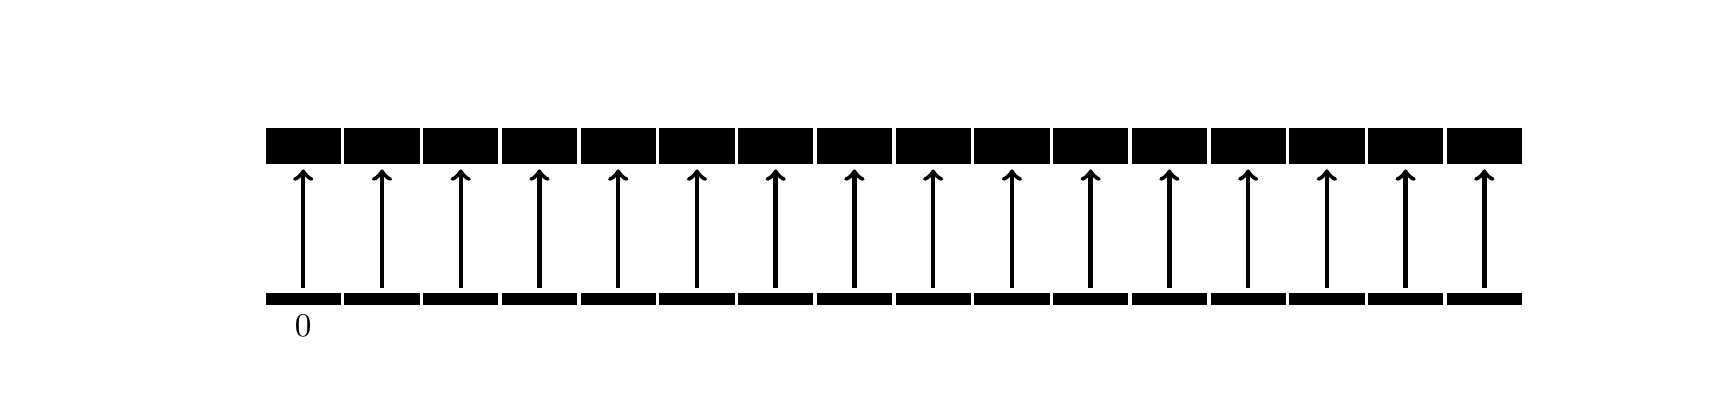
\begin{tikzpicture}

            % the frame
            \path[clip] (-3, -3) rectangle (18, 1.5);

            % the body
            \foreach \i in {0,...,15} {
                \draw[ultra thick, fill=black] ({\i+0.05}, -0.2) rectangle ({\i+0.95}, 0.2);
                \path[->, ultra thick] ({\i + 0.5}, -1.8) edge node {} ({\i+ 0.5}, -0.3);
            };

            % nat
            \foreach \i in {0,...,15} {
                \draw[ultra thick, fill=black] ({\i+0.05}, -2) rectangle ({\i+0.95}, -1.9);
            }

            % label
            \node[below, scale=1.2] at (0.5, -2) {$0$};
        \end{tikzpicture}
    \end{adjustbox}
\end{center}


It would be a shame if only a few of \lstinline|Numeral| can be converted from
natural numbers, and all that effort we have put into generalizing $ o $ will be
gone to waste.

However, if we consider converting natural numbers that starts from somewhere
other than $0$, then much more numeral systems will be applicable for \lstinline|fromℕ|.
Besides, functions and predicates that we have constructed such as \lstinline|increment|
and \lstinline|Continuous| will be useful


% Besides, we do not go all the way constructing things such as \lstinline|next-numeral| or
% \lstinline|increment| for nothing.

\begin{center}
    \begin{adjustbox}{max width=\textwidth}
        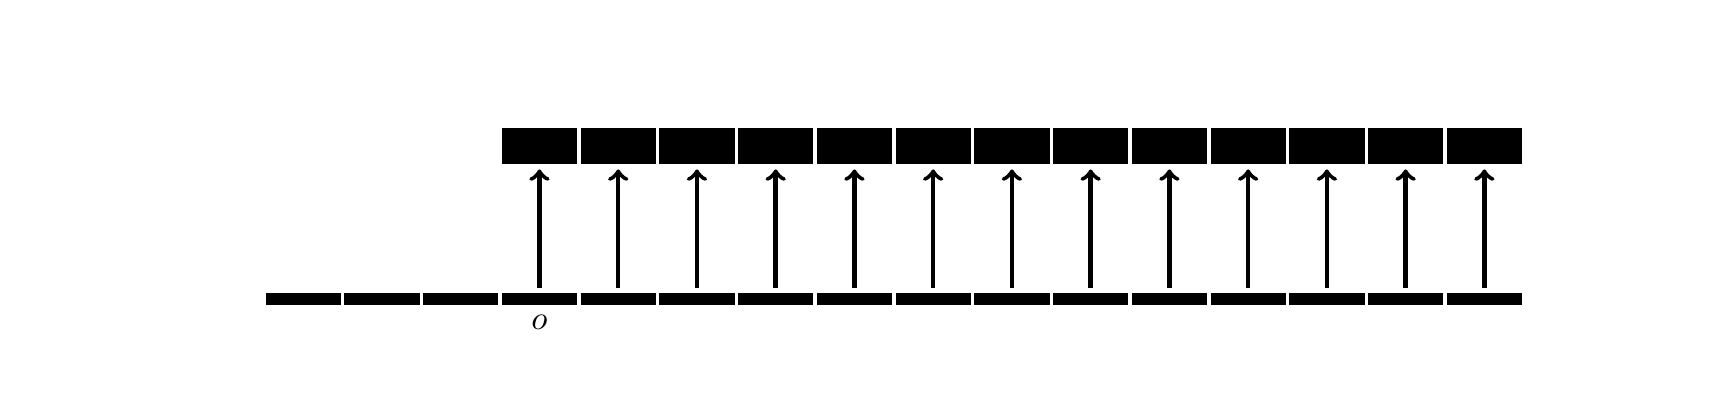
\begin{tikzpicture}

            % the frame
            \path[clip] (-3, -3) rectangle (18, 1.5);

            % the body
            \foreach \i in {3,...,15} {
                \draw[ultra thick, fill=black] ({\i+0.05}, -0.2) rectangle ({\i+0.95}, 0.2);
                \path[->, ultra thick] ({\i + 0.5}, -1.8) edge node {} ({\i+ 0.5}, -0.3);
            };

            % nat
            \foreach \i in {0,...,15} {
                \draw[ultra thick, fill=black] ({\i+0.05}, -2) rectangle ({\i+0.95}, -1.9);
            }

            % label
            \node[below, scale=1.2] at (3.5, -2) {$o$};

        \end{tikzpicture}
    \end{adjustbox}
\end{center}


% However, if we allow natural numbers to start from numbers other than $0$,





%
% It would be a shame


% It is straightforward to define \lstinline|fromℕ| only on the systems with
% a surjective \lstinline|⟦_⟧|.



%
% \begin{lstlisting}
% fromℕ : ∀ {b d}
%     → (n : ℕ)
%     → Numeral b (suc d) 0
% fromℕ zero = z ∙
% fromℕ (suc n) = z ∙
%
% {o = o}       n       p   with o ≟ n
% fromℕ               n       n≥o | yes eq = z ∙
% fromℕ {o = o}       zero    n≥o | no ¬eq = contradiction (≤0⇒≡0 o n≥o) ¬eq
% fromℕ {cont = cont} (suc n) n≥o | no ¬eq = 1+ {cont = cont} (fromℕ {cont = cont} n (≤-pred $ ≤∧≢⇒< n≥o ¬eq))
% \end{lstlisting}


% However, doing so would exclude systems with $ o \textgreater 0 $



% As we have seen, some instances of the evaluation function \lstinline|⟦_⟧|
% for systems like \lstinline|Numeral 10 5 0|, may not be surjective,
% and thus do not have an inverse function.
%
% For \lstinline|fromℕ|, an inverse function of \lstinline|⟦_⟧|, to be well-defined,
% its corresponding \lstinline|⟦_⟧| have to be surjective.


%
% % the intance of

 % to be well-defined,

% As we have seen, the evaluation function \lstinline|⟦_⟧| for some of the systems
% like \lstinline|Numeral 10 5 0|, may not be surjective.

% However, as an inverse function of \lstinline|⟦_⟧|, \lstinline|fromℕ| can only
% be well-defined when a certain instances of \lstinline|⟦_⟧| is

% the evaluation function \lstinline|⟦_⟧| for systems like
% \lstinline|Numeral 10 5 0| are not surjective, therefore it does not have an
% inverse function.
%
% For \lstinline|fromℕ| to be well-defined,







% Systems like \lstinline|Numeral 10 5 0| are not surjective, therefore the inverse



% We can allow only the numeral systems with surjective evaluation functions to be
% converted from natural numbers, but systems with $ o \textgreater 0 $ will not
% be qualified







\end{document}
